\chapter{Results and Discussion}

\section{Problem set}
The algorithm described receives output value by sending necessary input to the black-box functions. These are synthetic black-box functions whose global optimal solutions are known. These black-box functions vary in input parameters ranging from 1 to 300 variables and are classified in four categories based on whether they are convex or non-convex and whether these functions are smooth or non-smooth. The code for these functions are available as C files to be compiled at the Sahinidis Optimization Group website (http://archimedes.cheme.cmu.edu/?q=dfocomp).

\bigskip
\noindent
The number of problems for the four categories described is shown in Table \ref{tab:problemData}. The detailed overview of the problems evaluated based on number of variables given is seen in Figure \ref{fig:ProblemSet}.

\begin{table}[h]
\centering
\begin{tabular}{ | P{5cm} | P{5cm} |  }
 \hline
  \textbf{Problem Category}  & \textbf{Number of problems} \\
 \hline
 Non-Convex Non-Smooth & 17 \\
 Non-Convex	Smooth     & 236 \\
 Convex Non-Smooth     & 150 \\
 Convex Smooth         & 72 \\
  \hline
 \end{tabular}
\caption{Problem set overview}
\label{tab:problemData}
\end{table}


\begin{figure}
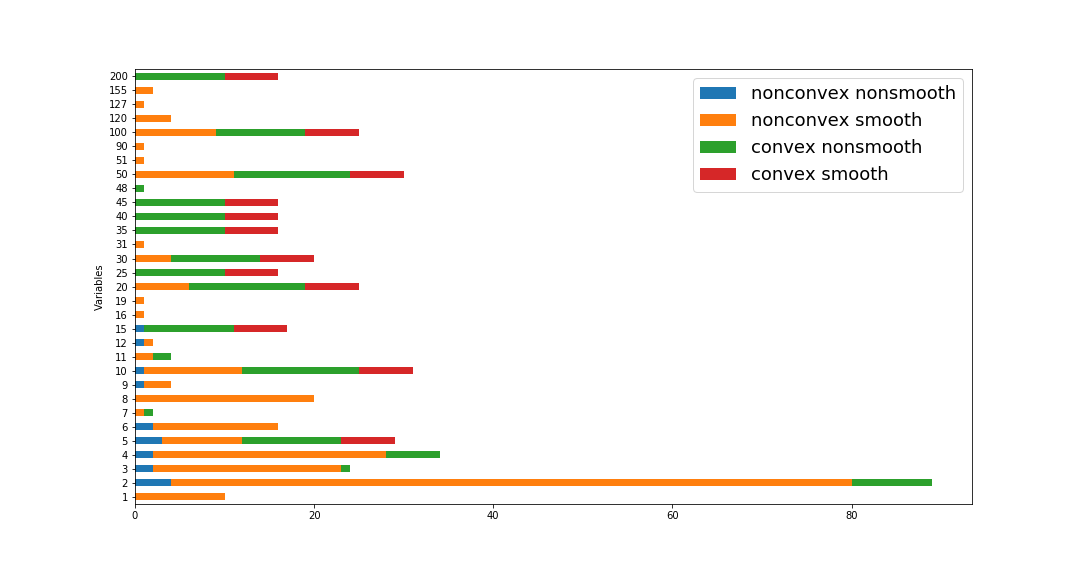
\includegraphics[width=0.9\textwidth]{Dataset_info.PNG}
\caption{Number of test problems based on type and number of variables}
\label{fig:ProblemSet}
\end{figure}

\section{Convergence criteria}
In these problems, reaching the exact global optima would require infinite function evaluations for the points to converge. So, in order to examine whether a given problem converged or not, following criteria were setup.

\subsection{Relative error}
The output values were compared based on relative error and if the relative error (RE) was less than $0.5\%$, then the problem is deemed to have converged. If y* is the global optima and $\^{y}$ is the present value, then the following expression would be true if the solution has converged.
\begin{center}
$RE(y^{\ast},\^{y}) = \displaystyle\frac{y^{\ast}-\^{y}}{\^{y}} \leq 0.5\%$
\end{center}


\subsection{Absolute error}

For the given set of problems, about half of them had an optimal solution value of zero or values tending to be zero in which case the relative error becomes undefined. For those cases, the absolute error values was instead used. Most of these problems had very high values in the range of $10^{10}$ to $10^{30}$ when the solution was far from optimal. Thus, for convergence, the convergence criteria was satisfied if the absolute error was less than one.

\subsection{Average Manhattan distance}
For some instances, the reported optimal y* values are different from the $\^{y}$ values even when the feature values are the same. Thus, instead of solely relying on the output values, proximity of the feature values with those of optimal solution was also analyzed. To normalize the distance value computed, the distance was normalized with the distance between the upper and lower bounds of that feature value, and the convergence of solution is checked by the below equation. For analysis, the Manhattan distance (MD) metric was selected since it is not biased towards the number of features. Using sum squared distances as the criteria here would make it less stringent on higher number of features.

\begin{center}% 
\mbox{\large\( %
MD(x) = \displaystyle\sum_{i=1}^M\frac{ |x^*_i - \^{x}_i | }{ x^{(UB)_i} – x^{(LB)_i} } \leq 0.01\%
\)} %
\end{center}

\noindent
where M is the total number of features in x.

\section{Experimental setup}
The computation for all the analysis was carried out on a 64-bit Intel 2.70 GHz processor in a Windows machine. The code for the models was run using Python 3.7. The same set of problems were tested in \cite{Rios2012} where there was a limit of 2,500 function evaluations in each run. Thus, same evaluation budget was reserved for analyzing the convergence.

\bigskip
\noindent
Some of the problems defined have no bounds, but since the sampling stage of the algorithm relies on bounds, all the variables for these problems were given bounds in the interval [-10000, 10000]. In order to tally the results, the starting point specified for use in the problem data was selected. After selecting the parameters, each problem was run only once and its performance compared.

\bigskip
\noindent
In order to assess the quality of the solutions obtained, the solutions returned by the algorithm against the globally optimal solution for each problem was analyzed as described in the previous section. 

\bigskip
\noindent
During the computations, the algorithm was able to receive only the output value based on the input feature values given. The algorithm itself calculated all other data, including the gradient of the response surface model built. 

\subsection{Hyperparameter settings}
The algorithm has various hyperparameters whose values were tweaked initially to obtain the ones that gave best performance. The momentum factor ($\beta$) was set to 0.9 based on research in this domain. The patience factor determines the exploratory versus exploitative trade-off in the algorithm. In the present work, it was set to three occurrences for all problems. The sampling domain was attenuated or augmented for the features selected in the cyclic approach using the scaling factor ($SF_i$) for the specific iteration number $i$. 

\begin{center}
$\displaystyle SF_i = SF_{i-1}\times \Big(\frac{Z_i}{Z_{i-1}} \Big)^p$    
\end{center}
    
\noindent
where $Z_i$ is the output value for the $i^{th}$ iteration and p was a constant set to 0.5. If the output is negative, the constant p was multiplied by -1. For the first iteration, the scaling factor for all features is initialized to 1. In some cases, the values of output might change signs from negative to positive or vice-versa. In such cases, if the values improved, then the scaling factor was halved and otherwise it was doubled.

\bigskip
\noindent
The most important hyperparameter to choose is the number of attributes to be modeled for the cyclic coordinate approach. This becomes an extremely challenging decision when the number of attributes increase over 30. The number of attributes selected for the present analysis is listed in the Table \ref{tab:HyperFeature}. Since the black-box function cannot pre-determine the convexity and smoothness of the problem, these hyperparameter settings were applied to all kinds of problems.
\begin{table}[h]
\centering
\begin{tabular}{ | P{4cm} | P{4cm} | P{4cm} |  }
 \hline
  \textbf{Total Features}  & \textbf{Sampled points}	& \textbf{Features selected} \\
 \hline
 1-2 & 20 & 1 \\
 3-6 & 20	& 2 \\
 7-15	& 25 & 3 \\
 16-30	& 30 & 4 \\
 50-100 & 30 & 6 \\
 110-130 & 50 & 12	\\
 \hline
 \end{tabular}
\caption{Number of samples and features selected per iteration }
\label{tab:HyperFeature}
\end{table}

\section{Illustrative example: camel6}
The  camel6 problem, an abbreviation for the ‘six-hump camel back' function as seen in the equation below, was used to demonstrate the convergence strategy employed by the algorithm.

\begin{center}
$\displaystyle f(x)= \Big(4 - 2.1x_1^2 = \frac{x_1^4}{3} \Big)x_1^2 + x_2x_1 + (4x_2^2-4)x_2^2$
\end{center}

\begin{figure}[t]%
    \centering
    \subfloat[Search in 1 dimension]{{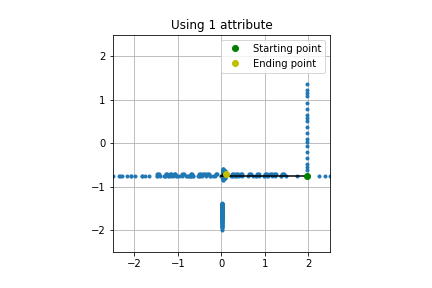
\includegraphics[width=8cm]{img/Camel6_1attr.png} }}%
    \subfloat[Search in 2 dimensions]{{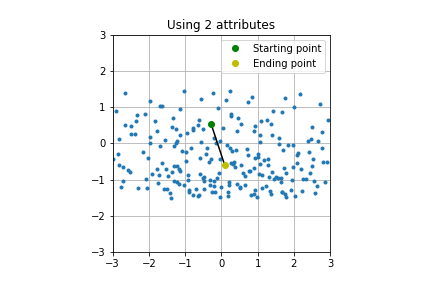
\includegraphics[width=8cm]{img/Camel6_2attr.png} }}%
    \caption{Comparison of sampling while the points converge for the camel6 problem}
    \label{fig:Camel6}
\end{figure}

\noindent
There are two global minima for this function with f(x*) = -1.0316, at x* = (0.0898, -0.7126) and (-0.0898, 0.7126) while the remaining four are local optima.
Using the algorithm, the problem was solved with one and two attributes respectively as seen in Figure \ref{fig:Camel6}.
When using one attribute, the problem starting from $x_0^{(1)}$ = (1.975301, -0.75768) converges to the point $\^{x}^{(1)}$ = (0.095951, -0.71191) with $f( \^{x}^{(1)})$ of -1.03147. 
Similarly, when using two attributes, the problem starting from $x_0^2 = (-0.2934, 0.5758)$ converges to the point $\^{x}^{(2)} = (0.0640, 0.7246)$ with $f(\^{x}^{(1)})$ of -1.03089. For both experiments, the convergence was achieved within the specified budget of 2500 function evaluations.

\section{Black-Box Problems}
This section compares the performance of this algorithm with those described in \cite{Rios2012}. The strategy for boosting the algorithm's performance using momentum was derived from \cite{Mukherjee2013} where it was referred to as the BOOM algorithm and the same term is referred to in the plots here. The results for this are computed at convergence while for the rest of the algorithms, the fraction was recorded only after 100, 200, 500, 1000, 2000 and 2500 evaluations. In these plots, the horizontal axis shows the progress of the algorithm as the number of function evaluations gradually reached 2,500.

\subsection{Computational results for convex problems}

% ConvexSmooth
Figure \ref{fig:ConvexSmooth} shows the fraction of convex smooth problems solved by each solver within the optimal tolerance specified. This algorithm solves about 45\% of the problems. The TOMLAB/GLCCLUSTER is the best solver in this category followed by MCS, solving about 75-80\% of the problems. 

\begin{figure}[h]
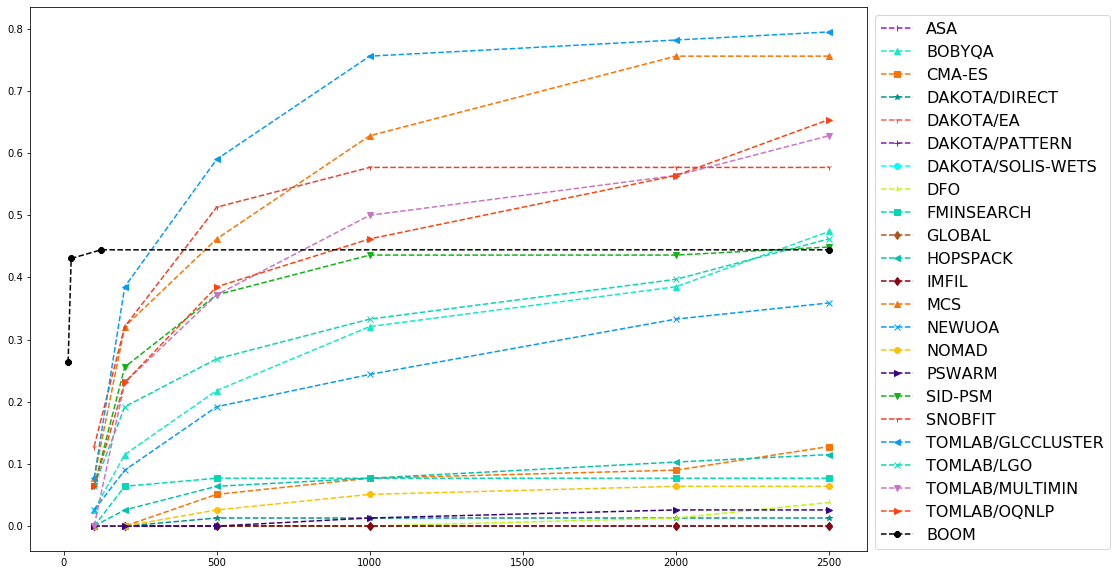
\includegraphics[width=0.9\textwidth]{img/cvx_sm.png}
\caption{Comparison of fraction of convex smooth problems solved as a function of number of function evaluations}
\label{fig:ConvexSmooth}
\end{figure}

% ConvexNonSmooth
\bigskip
\noindent
Figure \ref{fig:ConvexNonSmooth} shows the fraction of convex non-smooth problems solved. This algorithm solves close to 52\% of the problems while the solvers TOMLAB/GLCCLUSTER and TOMLAB/MULTIMIN follow closely, solving about 43\% of the problems. 

\begin{figure}
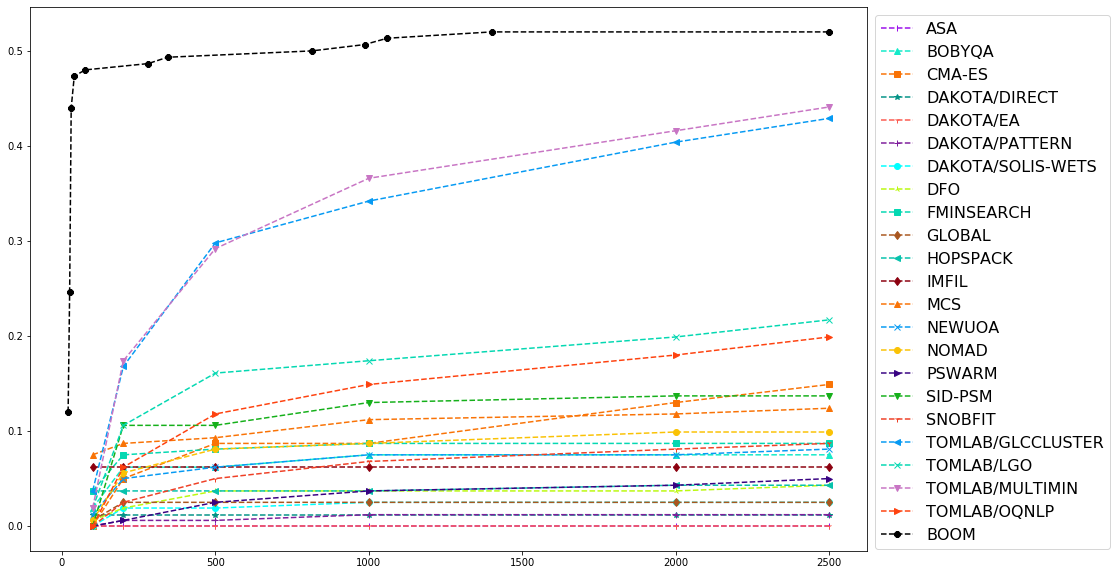
\includegraphics[width=0.9\textwidth]{img/cvx_nsm.png}
\caption{Comparison of fraction of convex non-smooth problems solved as a function of number of function evaluations}
\label{fig:ConvexNonSmooth}
\end{figure}

\subsection{Computational results for non-convex problems}
Figure \ref{fig:NonConvexSmooth} displays the solution progress for non-convex smooth problems. The present algorithm is able to solve about 67\% of the problems. The TOMLAB/MULTIMIN and TOMLAB/GLCCLUSTER are the only solvers to solve more than 70\% of the problems.

% NonConvexSmooth
\begin{figure}[h]
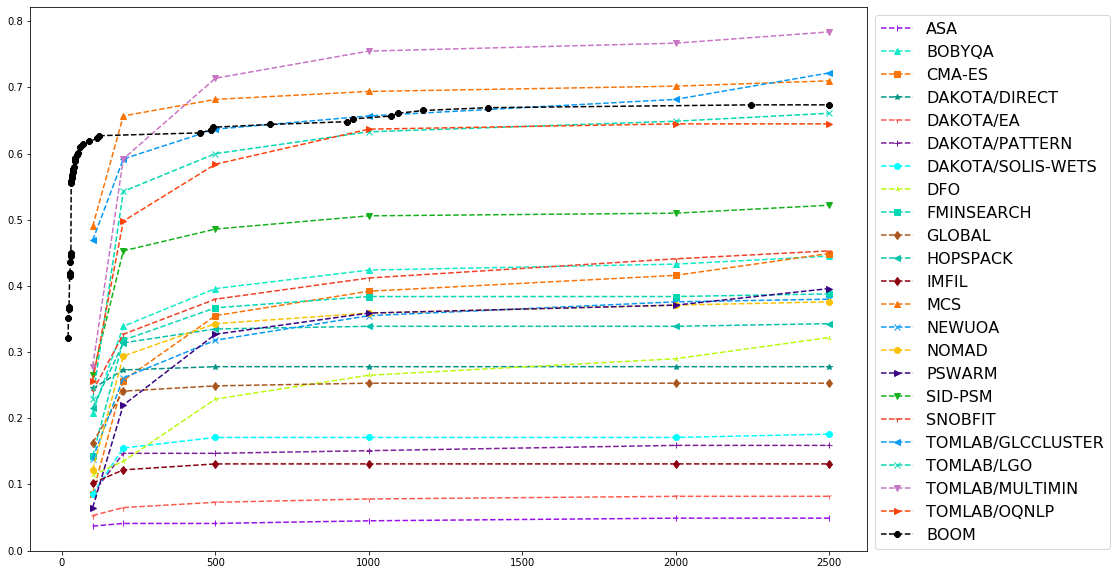
\includegraphics[width=0.9\textwidth]{img/ncvx_sm.png}
\caption{Comparison of fraction of non-convex smooth problems solved as a function of number of function evaluations}
\label{fig:NonConvexSmooth}
\end{figure}

\noindent
Figure \ref{fig:NonConvexNonSmooth} presents the fraction of non-convex non-smooth test problems. The present algorithm solves about 35\% of the problems. The TOMLAB/MULTIMIN solves 45\% of the problems followed by  TOMLAB/LGO solving 39\% of the problems.

\begin{figure}
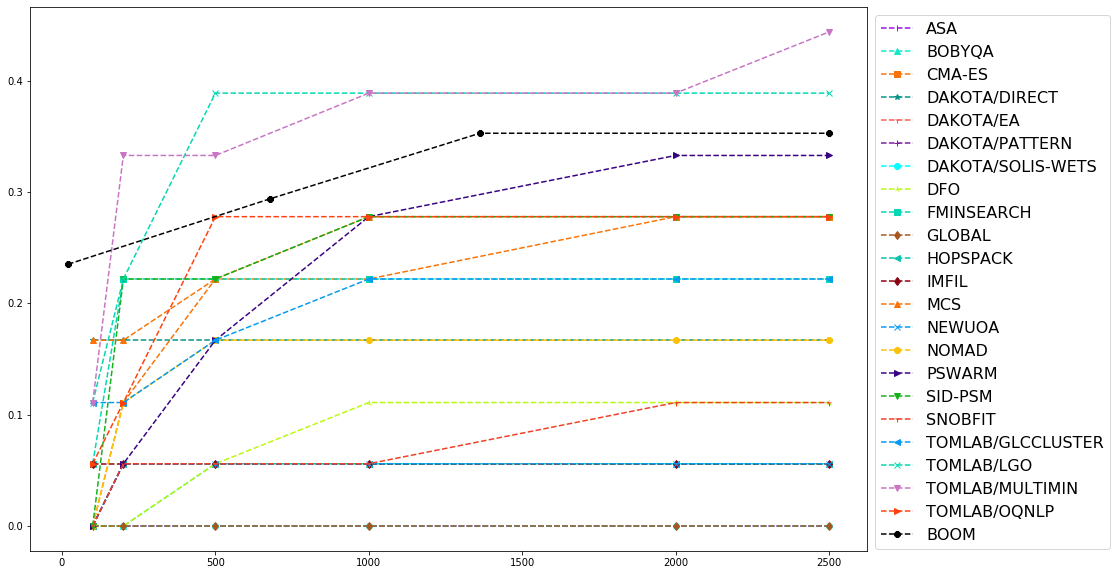
\includegraphics[width=0.9\textwidth]{img/ncvx_nsm.png}
\caption{Comparison of fraction of non-convex non-smooth problems solved as a function of number of function evaluations}
\label{fig:NonConvexNonSmooth}
\end{figure}

\subsection{Comparison of results}
In this analysis, it must be noted that the present algorithm was solved on 475 problems while rest of the solvers were used to solve all the 500 problems. From the plots, it can be observed that the algorithm converges for many problems initially. This is owing to the quasi-random sampling employed in finding a good starting point. Following this, the points quickly converge to the globally optimal solution using the block coordinate descent approach. Since many of the problems are in low dimensions, a high rate of convergence is attained early on. 

\bigskip
\noindent
However, finding a good initial point in higher dimensions is difficult. This reflects the fact that the algorithm must have the potential to improve and reach the global optima once an initial point is chosen. Recent studies using the ADAM optimizer have shown that using not only the first but also the second moment of the gradient are much more successful in reaching global optima. This is because the additional term helps in escaping the local optima whereas the implementation of the Nesterov Accelerated Gradient (NAG) is susceptible to getting stuck in local optima. In most cases, NAG may converge if fortuitously the momentum is in the direction of the global optima. Thus, calculation of Hessian matrix for the variables and incorporating it along with the first moment will help in increasing the convergence of the algorithm.

\section{Hidden Constrained problem}
As a special case, this algorithm was tested to solve a chemical process system which has a hidden constrained problem. The objective of this problem is to minimize the total energy consumption on a per day basis during LNG (Liquefied Natural Gas) Production. The problem was formulated on ASPEN HYSYS V10, which is a commercial process simulator for the chemical engineering industry. This simulator acts as the Black-Box function, returning the objective value for 8 variables in this system; 4 variables are the pressures at different locations and the remaining 4 are the composition variables (the fifth composition variable is automatically set based on the remaining 4 compositions). All of these functions were linked to the algorithm written in Python, receiving an output value from the simulators.

\begin{figure}[h]
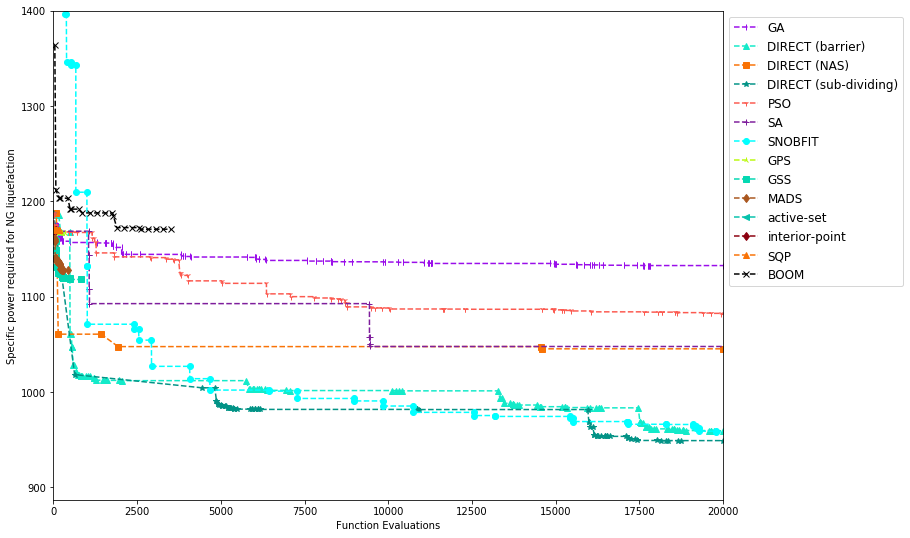
\includegraphics[width=0.9\textwidth]{img/ASPEN_problem.png}
\caption{Comparative plot of various solvers on the ASPEN HYSYS problem}
\label{fig:ASPEN_prob}
\end{figure}

\bigskip
\noindent
An analysis of this problem has been carried out in \cite{Na2017} which used a modified DIRECT algorithm that has been able to achieve the best possible solution till date. This paper contains the details of the problem, variables, and their lower and upper bounds. This problem was tested on a budget of 20,000 function evaluations, which has been the limit set by other algorithms solving this problem. 

\bigskip
\noindent
The plot of \ref{fig:ASPEN_prob} shows that the present algorithm converges on a local optima of $1170.8 \; kJ/kg-LNG$. The best solvers compared here obtaining solutions in the range of $950-970 \; kJ/kg-LNG$ were some modifications of the DIRECT (DIviding RECTangles) algorithm. Thus, the DIRECT algorithm is better at solving hidden constrained problems by dividing the search region into feasible spaces. In order to improve the solution in the present algorithm to move from local to global solution, modification to incorporate DIRECT algorithm can be carried out. Although DIRECT was not implemented in the present algorithm owing to the curse of dimensionality faced on using the DIRECT algorithm, future work on this algorithm can look into the adaptive block coordinate and DIRECT algorithm \cite{Tao2017} to help the algorithm to escape the local optima.